% !TEX encoding = UTF-8 Unicode 
%
% Use:
% magister / inzynier - for master thesis or engineering thesis
% druk / archiwum - for print version or archive version
% en - to translate template into english
% examples:
%\documentclass[inzynier,druk,en] - master thesis, print version, english
%\documentclass[magister,druk,en]{dyplom}
%\documentclass[magister,druk]{dyplom}

\documentclass[magister,druk]{dyplom}

\usepackage[utf8]{inputenc}
\usepackage{hyperref}

% Maximum section's depth.
\setcounter{secnumdepth}{4}

% Listings settings
\setminted{breaklines, 
frame=lines,           
framesep=3mm,          
baselinestretch=1.1,   
fontsize=\small,       
% linenos              % line numbering
}

\usepackage{lipsum}

% \faculty{Faculty of \dots}                   % Uncomment if applicable
\fieldofstudy{Kierunek z kodem spec., jeżeli dotyczy; np. Informatyka Stosowana (IO)}                          
\author{Imię i nazwisko autora}
\title{Tytuł pracy}
\supervisor{Tytuł, imię i nazwisko opiekuna pracy}
% \consultant{Consultant's name}               % Uncomment if applicable
% \specialisation{AAA}                         % Uncomment if applicable
\keywords{słowo1, słowo2, słowo3}	% 3-5 keywords  

\begin{document}

\maketitle

\abstract{
% English abstract 

\lipsum[1]

}{
% Abstract translated into Polish

\lipsum[2]

}

\tableofcontents

% !TEX encoding = UTF-8 Unicode 
% !TEX root = praca.tex

\chapter*{Wprowadznie}

Niniejszy szablon jest adaptacją szablonu opracowanego przez Pana Wojciecha Myszkę (patrz https://kmim.wm.pwr.edu.pl/myszka/projekty).

Został przetestowany w następujących narzędziach:
\begin{itemize}
\item Overleaf.com -- wersja on-line; nie jest wymagana instalacja
\item TeXStudio/TeXLive oraz TeXStudio/MiKTeX oraz TeXWorks/MiKTex
\end{itemize}

Użycie pełnej wersji może wymagać (np. dla zestawu TeXWorks/MikTeX):
\begin{itemize}
\item instalacji Python 2.7+ wraz z pakietem Pygments; ścieżki do obu narzędzi powinny być ustawione w zmiennej środowiskowej PATH -- pakiet jest używany do kolorowania słów kluczowych w listingach języków programowania
\item w środowisku Latex należy włączyć opcję -shell-escape  -- jest wymagana dla pakietu ``minted'' Latexa 
\end{itemize}

\section*{Cel pracy}

\lipsum[5]

\section*{Zakres pracy}

\lipsum[6]

% !TEX encoding = UTF-8 Unicode 
% !TEX root = praca.tex

\chapter{Tytuł rozdziału I}

W książce \cite{docker_compose_reference} \dots



\section{Rysunki}

\begin{figure}
\centering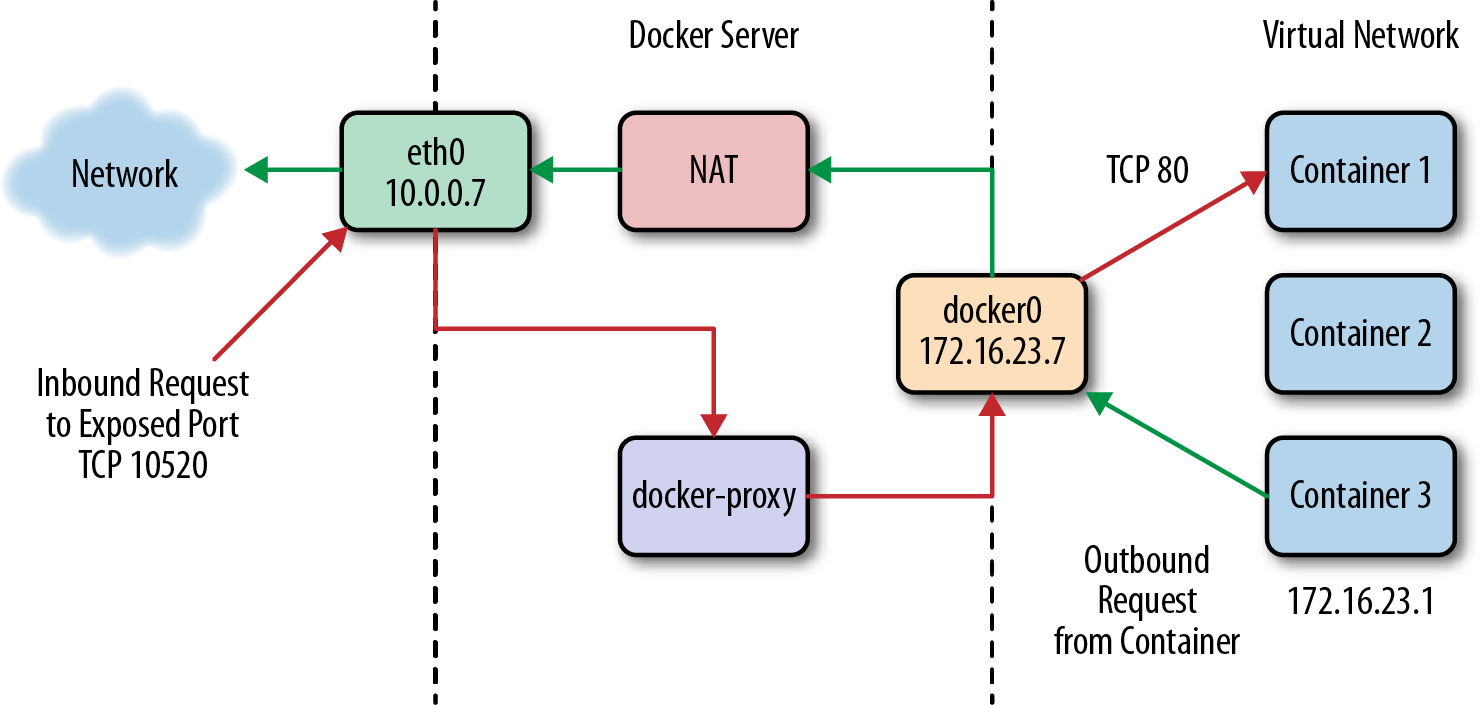
\includegraphics[width=.6\textwidth]{img/swarm-network}
\caption{Sieć dokera \cite{docker_compose_reference}}  \label{rys:network}
\end{figure}

Na rysunku \ref{rys:network} \dots


\subsection{Dwa rysunki obok siebie}

\begin{figure}[ht] 
	\centering
	\begin{minipage}[b]{0.45\textwidth}
		\centering
\includegraphics[width=0.9\textwidth]{img/kotek} % left figure
		\caption{Lewy rysunek}\label{fig:lewy}
	\end{minipage}
	\begin{minipage}[b]{0.45\textwidth}
		\centering
		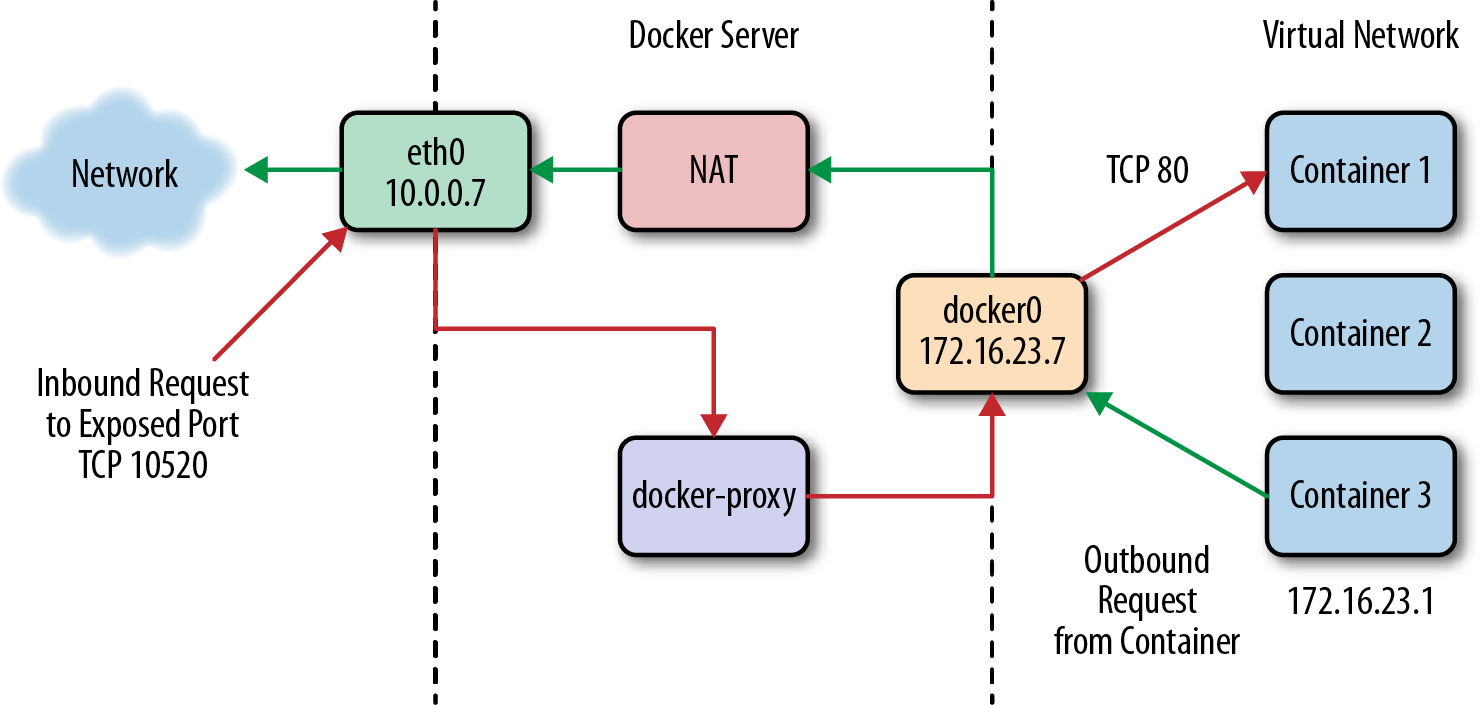
\includegraphics[width=0.9\textwidth]{img/swarm-network} % right figure
		\caption{Prawy rysunek}\label{fig:prawy}
	\end{minipage}
\end{figure}

Na rysunkach \ref{fig:lewy} i \ref{fig:prawy} \dots


\section{Tabele}

W tabeli \ref{table:table1} \dots

\begin{table}
\centering\caption{Tytuł tabeli (patrz dodatek~\ref{app1}) \label{table:table1}}
\begin{tabular}{|l|l|l|}% table alignment -> l c r - left, center, right
\hline
Pierwszy & Drugi & Trzeci \\
\hline
Pierwszy & Drugi & Trzeci \\
\hline
\end{tabular}
\end{table}

\subsection{Równania}

\begin{equation}
\sum_{i=1}^{\infty}a_i
\label{eq:myEquation}
\end{equation}

W równaniu \ref{eq:myEquation} \dots

\section{Listingi}

Na listingu \ref{listing:myListing} \dots

% replace {c} with the appropriate language
\begin{listing}
\begin{minted}{c}  
int main()
{
   int a=2*3;
   printf("**Ala ma kota\n**");
   while(!I2C_CheckEvent(I2C1, I2C_EVENT_MASTER_MODE_SELECT)); /* EV5 */
   return 0;
}
\end{minted}
\caption{Język C} \label{listing:myListing}
\end{listing}



% !TEX encoding = UTF-8 Unicode 
% !TEX root = praca.tex

\chapter*{Podsumowanie}

\lipsum[17]



% Bibliography
\bibliographystyle{dyplom}
\bibliography{bibliography}

% Lists of figures, listings, tables
\listoffigures
\listoflistings
\listoftables

% Appendices - comment out if not applicable
\appendixpage
\appendix
\chapter{Dodatek 1}\label{app1}

\lipsum[20]

\end{document}
